\documentclass[svgnames,final]{beamer}
\usepackage{etex}
\usepackage{multirow}
\mode<presentation> {
    \usetheme{I6dv}
}
\usepackage[utf8]{inputenc}
\usepackage[T1]{fontenc}
\usepackage[english]{babel}
\usepackage{amsmath,amsfonts,amsthm}
\usepackage{mathtools}
\usepackage{lmodern}
\usepackage{booktabs}
\usepackage[orientation=landscape,size=a0,scale=1.4]{beamerposter}
\usepackage{pgfplots}
\pgfplotsset{compat=1.9}
\usepackage{tikz}
\usetikzlibrary{positioning,plotmarks,calc,arrows,decorations.markings,intersections,backgrounds}
\usepackage{graphicx}
\usepackage{xypic}
\usepackage{subfigure}
\graphicspath{{./images/}}

\newcommand{\normal}{\mathcal{N}}
\newcommand{\muhat}{\widehat{\mu}}

\newcommand{\red}[1]{\textcolor{red}{#1}}
\newcommand{\green}[1]{\textcolor{Green}{#1}}
\newcommand{\blue}[1]{\textcolor{blue}{#1}}
\newcommand{\ve}{\varepsilon}
\newcommand{\eps}{\ve}
\newcommand{\Otilde}{\widetilde{O}}
\newcommand{\poly}{\mathrm{poly}}
\newcommand{\dtv}{d_{\mathrm{TV}}}
\newcommand{\thres}{\mathrm{Thres}}
\newcommand{\tail}{\mathrm{Tail}}
\newcommand{\hood}{\mathcal{S}}
\newcommand{\E}{\mathbb{E}}

\DeclareMathOperator*{\argmin}{arg\,min}

\renewcommand{\arraystretch}{1.4}
\newcommand{\calG}{\mathcal{G}}
\newcommand{\calD}{\mathcal{D}}
\newcommand{\R}{\mathbb{R}}
\newcommand{\TV}{\mathrm{TV}}
\newcommand{\I}{\mathbb{I}}

\newcommand{\tplr}[1]{\hspace{.8cm}#1\hspace{.8cm}}

\newcommand{\specialcell}[2][c]{%
  \begin{tabular}[#1]{@{}c@{}}#2\end{tabular}}


\title{EC521 - Cybersecurity Final Project: Open Source INTelligence (OSINT) Lab Generation}
\author{Maha Ashour, Jack Belmont, Pierre-Fran\c{c}ois Wolfe}
\institute{\textit{Boston University, College of Engineering}}

\begin{document}
\addtobeamertemplate{headline}{} 
{\begin{tikzpicture}[remember picture, overlay]
     \node [anchor=north east, inner sep=1.25cm, outer sep=1.25cm]  at (current page.north east)
     {
\includegraphics[height=5cm]{bu}};
  \end{tikzpicture}}

\begin{frame}
\vspace{-.5cm}
\begin{columns}[T]
\begin{column}{.3\linewidth}
\begin{block}{\large \textbf{\begin{center}Goals\end{center}}}
Lab generation project 
\begin{itemize}
\item Open Source INTelligence (OSINT) for identifying vulnerabilities
\item Introduce useful tools
\item Provide an interesting and ethical learning scenario
\item Build lab infrastructure: vulnerable webserver, synthetic datasets, challenges, etc.
\end{itemize}
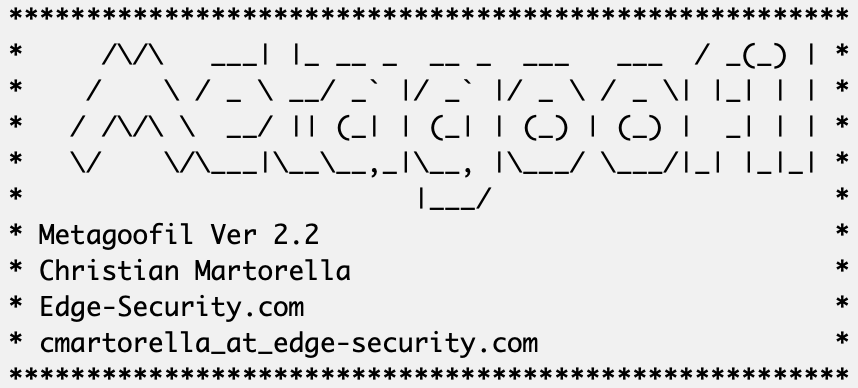
\includegraphics[scale=0.6]{metagoofil}
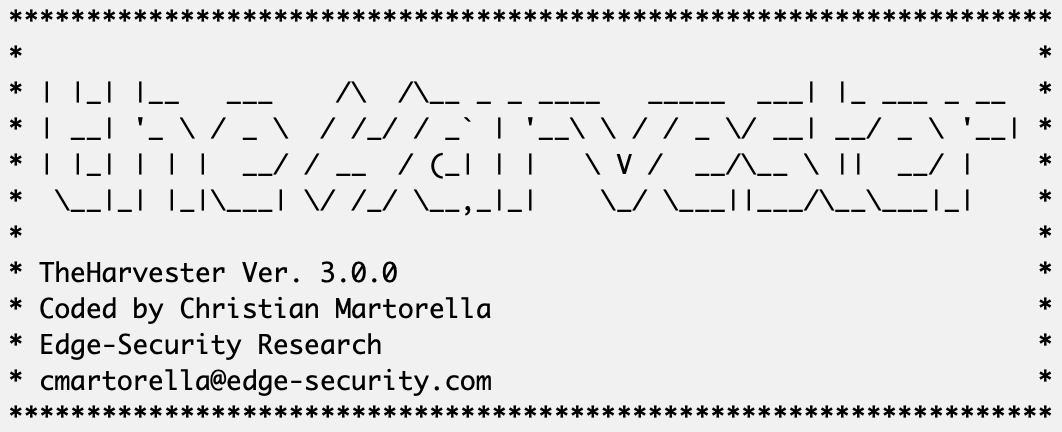
\includegraphics[scale=0.54]{theharvester}

\includegraphics[scale=0.3]{h8mail}

\includegraphics[scale=0.6]{maltego}
\end{block}

\begin{block}{\large \textbf{\begin{center}OSINT Cycle\end{center}}}
 
\begin{itemize}
\item Collect (gathering)
\item Process (data validation)
\item Exploit (determine value of information)
\item Produce (consumable/usable data)
\end{itemize}
\end{block}

\begin{block}{\large \textbf{\begin{center}Maltego\end{center}}}
\begin{itemize}
\item Data Mining Tool
\item Direct Graphs for Link Analysis
\item Relationship Analysis
\item Transforms for streamlined searching
\end{itemize}
\end{block}

\begin{block}{\large \textbf{\begin{center}Other Tools\end{center}}}
\begin{itemize}
\item \textbf{theHarvester}
\begin{itemize}
\item Input: Web domain and data source (ex: bing, linkedin, shodan)
\item Output:  Report with emails, subdomains, hosts, employee names, open ports, etc.
\item Method: Gathers public information about domain using custom python scripts for each data source
\end{itemize}
\item \textbf{h8mail}
\begin{itemize}
\item Input: [List of] email(s)
\item Output: Passwords - hashed or plain text
\item Method: Looks through “breach compilation” to find match
\end{itemize}
\item \textbf{Metagoofil}
\begin{itemize}
\item Input: Web domain
\item Output: Report with usernames, software/server versions, other info
\item Method: Uses Google search to gather document metadata from a given domain
\end{itemize}
\end{itemize}
\end{block}

\end{column}

\begin{column}{.3\linewidth}

\begin{block}{\large \textbf{\begin{center}Maltego: Custom Transforms\end{center}}}
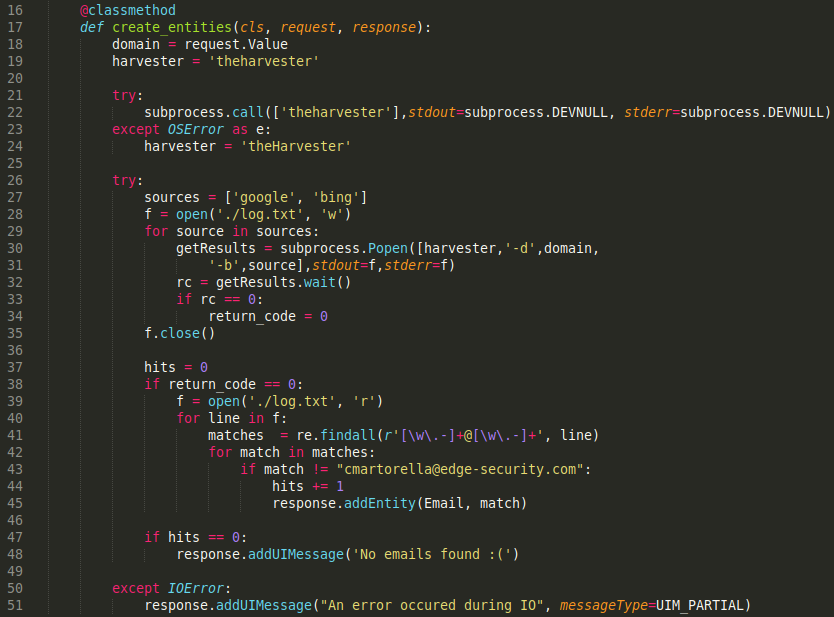
\includegraphics[scale=1.15]{transform}
\end{block}

\vspace{1.5cm}
\begin{block}{\large \textbf{\begin{center}Maltego: Network Analysis\end{center}}}
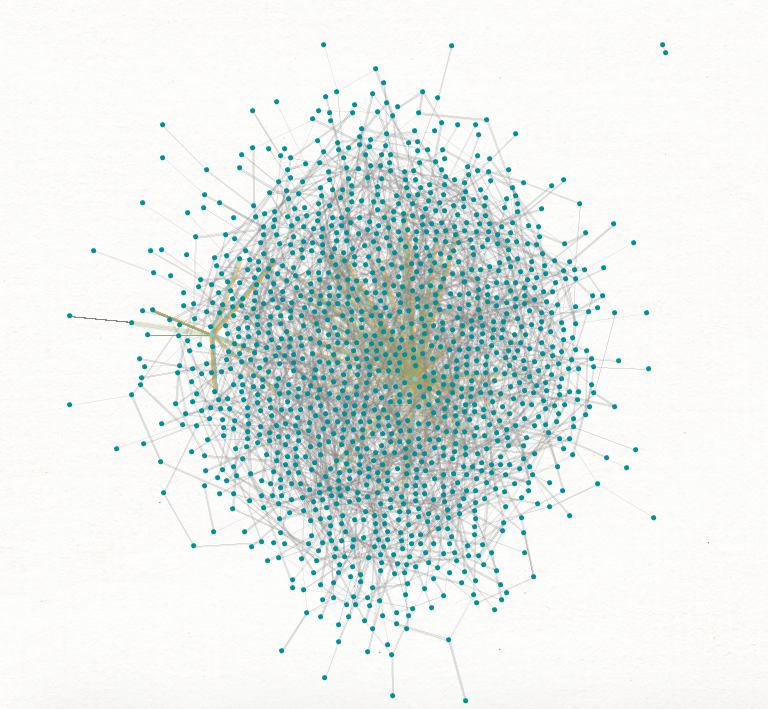
\includegraphics[scale=1.25]{network}
\end{block}
\end{column}

\begin{column}{.31\linewidth}

\begin{block}{\large \textbf{\begin{center}Vulnerable Webserver\end{center}}}
\textbf{Features}
\begin{itemize}
\item Login page with "Forgot my password" function
\end{itemize}
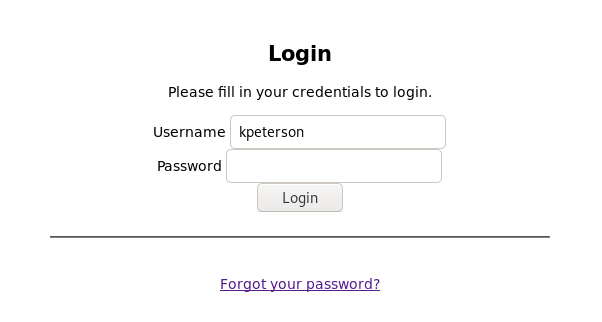
\includegraphics[scale=1.65]{login}
\begin{itemize}
\item File download	
\end{itemize}
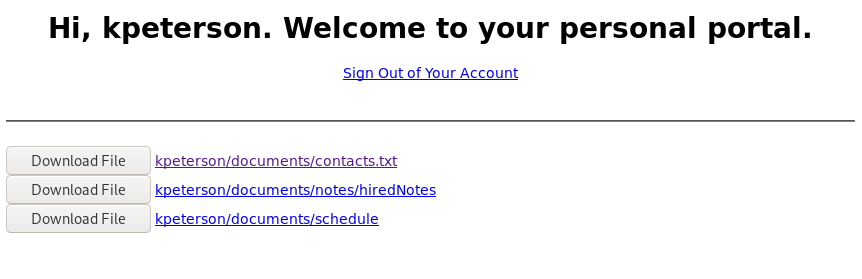
\includegraphics[width=\textwidth]{download}
\end{block}

\vspace{1cm}
\begin{block}{\large \textbf{\begin{center}Capture The Flag (CTF)\end{center}}}
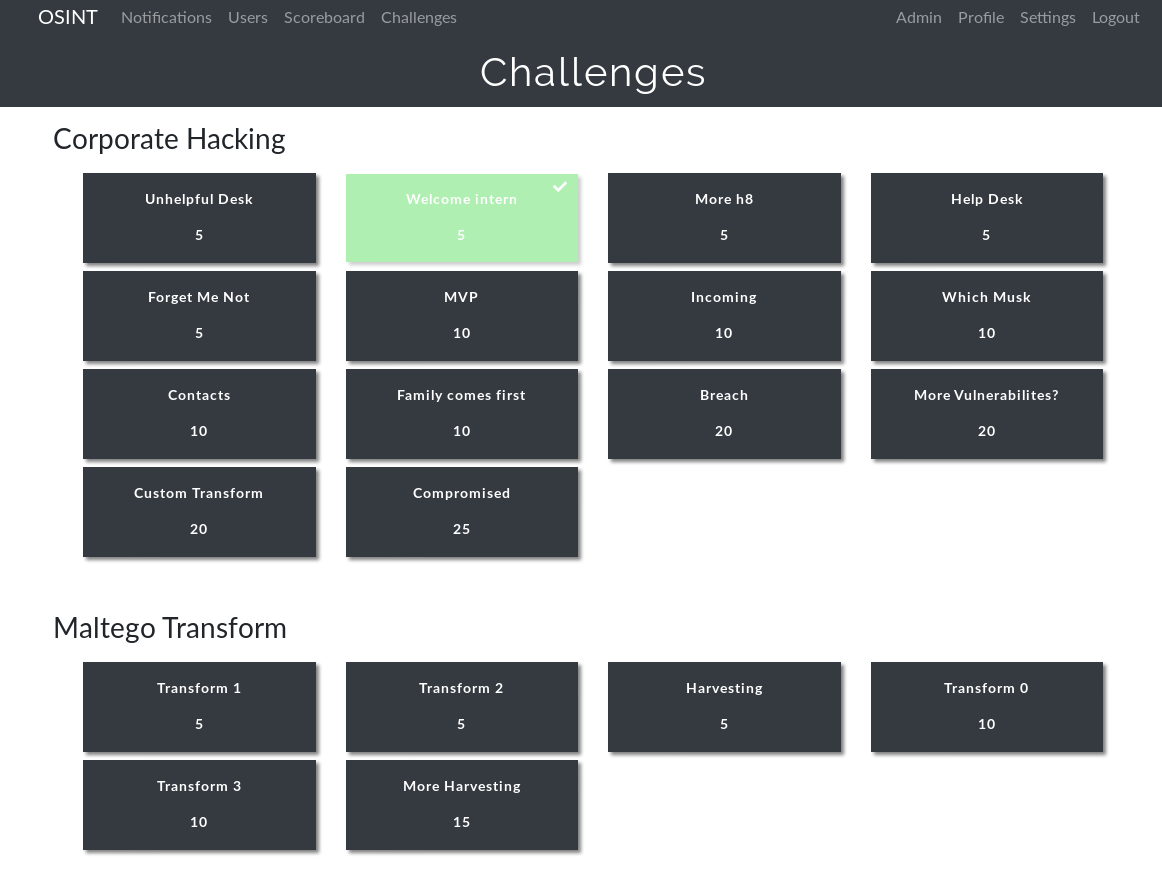
\includegraphics[scale=1.2]{ctf}
\end{block}
\vspace{-.6cm}
\end{column}
\end{columns}
\end{frame}
\end{document}
